\documentclass[10 pt,usenames,dvipsnames, oneside]{article}
\usepackage{../../../modelo-ensino-medio}



\begin{document}

\begin{center}
  \begin{minipage}[l]{3cm}

\includegraphics[width=2cm]{logo}    
\end{minipage}\hfill
\begin{minipage}[r]{.8\textwidth}
 {\Large \scshape Atividade: De 8 em 8 horas}  
\end{minipage}
\end{center}
\vspace{.2cm}

\ifdefined\prof
%Habilidades da BNCC
\begin{objetivos}
\item \textbf{EM13MAT508} Identificar e associar progressões geométricas (PG) a funções exponenciais de domínios discretos, para análise de propriedades, dedução de algumas fórmulas e resolução de problemas.
\end{objetivos}

%Caixa do Para o Professor
\begin{goals}
%Objetivos específicos
\begin{enumerate}
\item Deduzir a expressão que dá a soma dos termos de uma PG finita.

\end{enumerate}

\tcblower

%Orientações e sugestões
\begin{itemize}
\item Faça, caso julgue conveniente, a construção dessas tabelas em uma planilha eletrônica.

\begin{figure}[H]
\centering
\noindent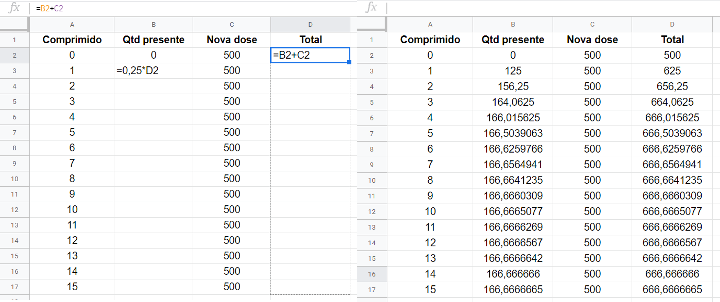
\includegraphics[width=\linewidth]{planilhaPG.png}
\end{figure}
\end{itemize}
\end{goals}

\bigskip
\begin{center}
{\large \scshape Atividade}
\end{center}
\fi

Você recebeu do médico a indicação de tomar o analgésico e antitérmico Paracetamol, 1 comprimido de 500mg, 3 vezes ao dia (de 8 em 8 horas) por 5 dias. Ao fazer uma pesquisa na internet você descobre que a meia-vida desse remédio é de 4 horas, isto é, que nesse intervalo de tempo, seu corpo consegue eliminar $50\%$ da quantidade de Paracetamol presente no seu corpo.

\begin{enumerate}

\item{}
Qual a porcentagem da dose ingerida estará no seu corpo $8$ horas após a primeira ingestão?

\item{}
Considerando que após $8$ horas, uma nova dose igual a inicial será ingerida, qual a quantidade total da substância no seu sangue?

\item{}
Organize os valores em uma tabela, e descubra a quantidade de paracetamol no seu sangue ao final de $24$ horas imediatamente antes de você tomar o novo comprimido.

%\begin{figure}[H]
%\centering
%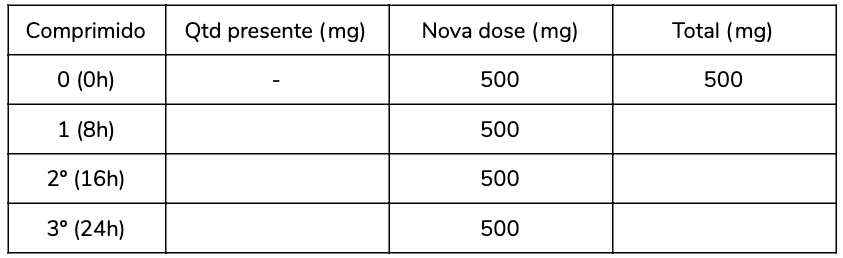
\includegraphics[width=300bp]{tabela1_oito_oito_horas.png}
%\end{figure}

\begin{center}
	\begin{tabular}{|c|c|c|c|}
		\hline
		\tcolor{Comprimido} & \tcolor{Quant. presente (mg)} & \tcolor{Nova dose (mg)} & \tcolor{Total (mg)} \\ \hline
		1 (0h)     & 0                   & 500            & 500        \\ \hline
		2 (8h)     &                     & 500            &            \\ \hline
		3 (16h)    &                     & 500            &            \\ \hline
		4 (24h)    &                     & 500            &            \\ \hline
	\end{tabular}
\end{center}

\item{}
Vamos generalizar: complete a tabela a seguir considerando a variável $d$ para a dose e $q$ para o fator de decaimento quaisquer.

%\begin{figure}[H]
%\centering
%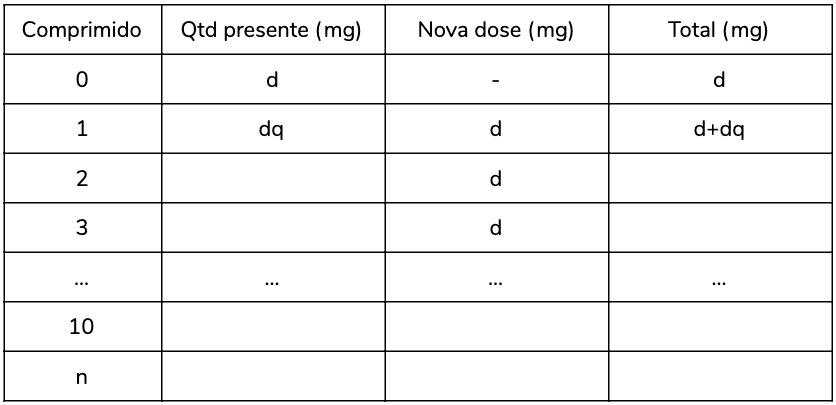
\includegraphics[width=300bp]{tabela2_oito_oito.png}
%\end{figure}
\begin{center}
	\begin{tabular}{|c|c|c|c|}
		\hline
		\tcolor{Comprimido} & \tcolor{Quant. presente (mg)} & \tcolor{Nova dose (mg)} & \tcolor{Total (mg)} \\ \hline
		1          & 0                   & $d$            & $d$        \\ \hline
		2          & $dq$                & $d$            & $d+dq$     \\ \hline
		3          &                     & $d$            &            \\ \hline
		$\cdots$   & $\cdots$            & $\cdots$       & $\cdots$   \\ \hline
		10         &                     & $d$            &            \\ \hline
		$\cdots$   & $\cdots$            & $\cdots$       & $\cdots$   \\ \hline
		n          &                     & $d$            &            \\ \hline
	\end{tabular}
\end{center}

\item{}
Para saber a quantidade de substância no sangue logo após tomar o último comprimido sem precisar calcular todas as etapas, Matheus pensou da seguinte maneira:

\begin{quote}
O último comprimido é o 15º (3 por dia, durante 5 dias). Pelo que vi na última tabela, a quantidade total de substância no meu sangue logo após ingeri-lo pode ser expressa por
\[
S=d+dq+dq^2+\cdots +dq^{14}+dq^{15}
\]
Se deixar passar o mesmo intervalo de tempo que estava habituado terei no meu sangue
\[
Sq=dq+dq^2+dq^3+\cdots +dq^{15}+dq^{16}
\]
E essas duas expressões têm quase todos os termos iguais! Se subtrair uma da outra, vou obter
\[
S-Sq=d-dq^{16}
\]
\[
S(1-q)=d(1-q^{16})
\]
\[
S=\dfrac{d(1-q^{16})}{1-q}
\]
Daí consigo calcular o valor de S, que era o que se desejava saber!

\end{quote}

Utilize o raciocínio do Matheus e os dados do Paracetamol (itens a, b e c) para calcular a quantidade de substância no seu sangue ao ingerir o último comprimido.

\end{enumerate}

\ifdefined\prof
\begin{solucao}

\begin{enumerate}
\item $25\%$
\item $125+500=625$mg
\item
\adjustbox{valign=t}
{
\begin{tabular}{|c|c|c|c|}
\hline
\tcolor{Comprimido} & \tcolor{Quant. presente (mg)} & \tcolor{Nova dose (mg)} & \tcolor{Total (mg)} \\ 
\hline
1 (0h) & --- & $500$ & $500$ \\ 
\hline
2 (8h) & $125$& $500$ & $625$ \\ 
\hline
3 (16h) & $181{,}25$ & $500$ & $681{,}25$ \\ 
\hline
4 (24h) & $170{,}31$ & $500$ & $670{,}31$ \\ 
\hline
\end{tabular}
}

\item 
\adjustbox{valign=t}
{\setlength\tabcolsep{2.5pt}
\begin{tabular}{|c|c|c|c|}
\hline
\tcolor{Comprimido} & \tcolor{Quant. presente (mg)} & \tcolor{Nova dose (mg)} & \tcolor{Total (mg)} \\ 
\hline
0 & $d$ & --- & $d$ \\ 
\hline
1 & $dq$ & $d$ & $d+dq$ \\ 
\hline
2 & $q(d+dq)$ & $d$ & $d+dq+dq^2$\\ 
\hline
3 & $q(d+dq+dq^2)$ & $d$ & $d+dq+dq^2+dq^3$\\
\hline
$\cdots$ & $\cdots$ & $\cdots$ & $\cdots$ \\ 
\hline
10 & $q(d+dq+\cdots+dq^9)$ & $d$ & $q(d+dq+\cdots+dq^10)$ \\ 
\hline
$\cdots$ & $\cdots$ & $\cdots$ & $\cdots$ \\ 
\hline
$n$ & $q(d+dq+\cdots+dq^{n-1})$ & $d$ & $q(d+dq+\cdots+dq^n)$ \\ 
\hline
\end{tabular}
}

\item $S=500\dfrac{1-0{,}25^{16}}{1-0{,}25}=666{,}66$mg
\end{enumerate}

\end{solucao}
\fi

\end{document}